\documentclass{beamer}
%\documentclass[handout,t]{beamer}

\batchmode
% \usepackage{pgfpages}
% \pgfpagesuselayout{4 on 1}[letterpaper,landscape,border shrink=5mm]

\usepackage{amsmath,amssymb,enumerate,epsfig,bbm,calc,color,ifthen,capt-of,multimedia,hyperref}

\usetheme{Berlin}
\usecolortheme{sustech}

\title{Reinventing the Wheel: Publishing High-quality Slides}
\author{Fan Jiang}
\institute{Southern Univ. of Science and Technology (SUSTech)}
\date{\today}

\pgfdeclareimage[height=0.5cm]{sustech-logo}{sustech-logo.pdf}
\logo{\pgfuseimage{sustech-logo}\hspace*{0.3cm}}

\AtBeginSection[]
{
  \begin{frame}<beamer>
    \frametitle{Outline}
    \tableofcontents[currentsection]
  \end{frame}
}
\beamerdefaultoverlayspecification{<+->}
% -----------------------------------------------------------------------------
\begin{document}
% -----------------------------------------------------------------------------

\frame{\titlepage}

\section[Outline]{}
\begin{frame}{Outline}
  \tableofcontents
\end{frame}

% -----------------------------------------------------------------------------
\section{Introduction}
\subsection{Who are we?}
\begin{frame}{Who are we?}
  \begin{columns}[T] % align columns
    \begin{column}<0->{.40\textwidth}
      \begin{figure}[thpb]
        \centering
        \resizebox{1\linewidth}{!}{
        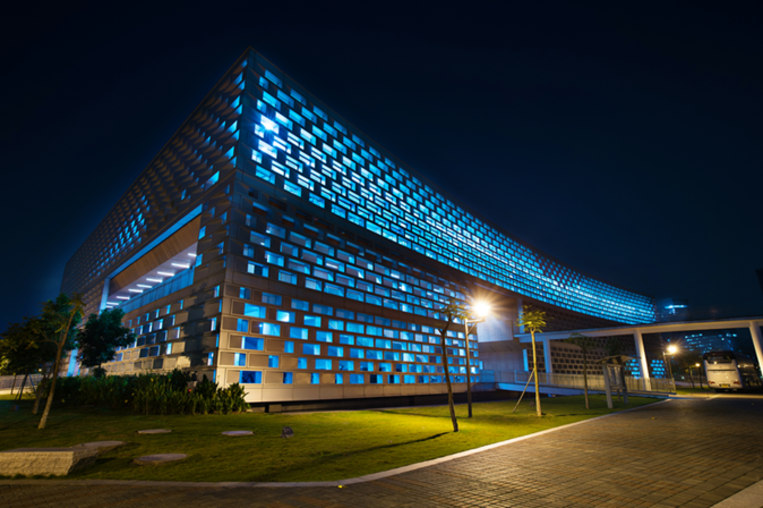
\includegraphics{figures/sustech.pdf}
        }
        %\includegraphics[scale=1.0]{figurefile}
        \caption{SUSTech Campus}
        \label{fig:campus}
      \end{figure}
    \end{column}%
    \hfill%
    \begin{column}<0->{.65\textwidth}
      \begin{itemize}
        \item<1-> Southern University of Science and Technology (SUSTech)
        \begin{itemize}
          \item<1-> Center of China's Education Reform
        \end{itemize}
        \item<2-> Shenzhen, the city of Makers
        \begin{itemize}
          \item<2-> The center of innovation in China
        \end{itemize}
      \end{itemize}
    \end{column}%
  \end{columns}
\end{frame}
\subsection{Problem Statement}
\begin{frame}{Problem scenario}
  Getting things done is difficult
  \begin{itemize}
    \item Human beings subject to their natural tendency to procrastinate
    \item Efforts are often in pure vain while hope is nowhere to be seen
    \item You do not have a girlfriend :)
  \end{itemize}
\end{frame}
\begin{frame}{State of the art}
  \begin{itemize}
    \item Current anti-procrastination systems lack raw force
    \begin{itemize}
      \item Pomodoro, GTD, etc.
    \end{itemize}
    \item Raw force are often misused and in the wrong hands
    \item People usually try to avoid punishment by telling lies
  \end{itemize}
\end{frame}
% -----------------------------------------------------------------------------
\section{System Design}
\subsection{System Architecture}
\begin{frame}{System architecture}
  \begin{columns}[T] % align columns
    \begin{column}<0->{.48\textwidth}
      \begin{figure}[thpb]
        \centering
        \resizebox{1\linewidth}{!}{
        
\includegraphics{figures/test.pdf}
        }
        %\includegraphics[scale=1.0]{figurefile}
        \caption{System components}
        \label{fig:system}
      \end{figure}
    \end{column}%
    \hfill%
    \begin{column}<0->{.48\textwidth}
      \begin{itemize}
        \item Electric Chair: Punishment
        \item Sensor: Detect behavior
        \item Handcuffs: Raw confinement
      \end{itemize}
    \end{column}%
  \end{columns}
\end{frame}
\begin{frame}{Tracking Results}
  \begin{columns}[T] % align columns
    \begin{column}<0->{.48\textwidth}
    \begin{figure}[thpb]
      \centering
      \resizebox{\linewidth}{!}{
      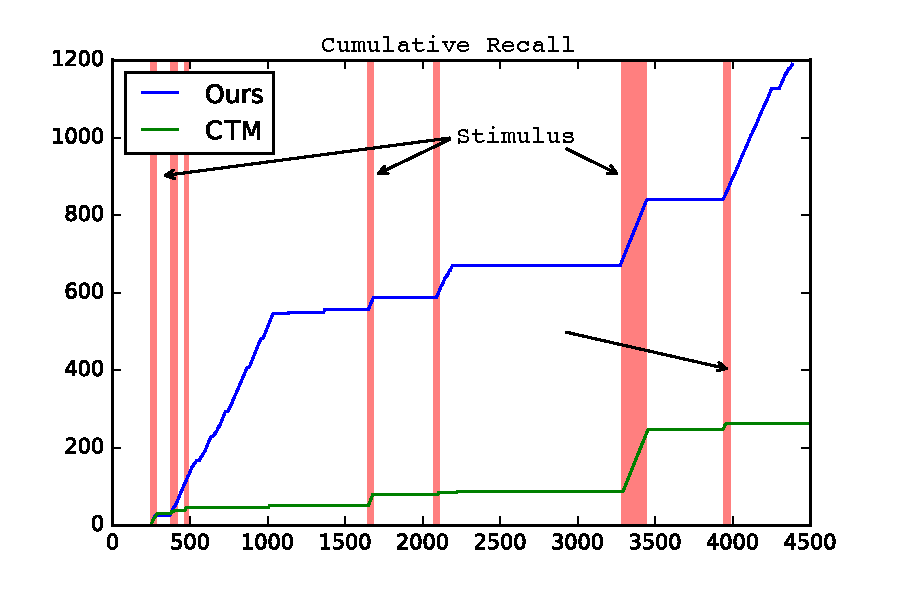
\includegraphics{figures/loss.pdf}
      }
      %\includegraphics[scale=1.0]{figurefile}
      \caption{Effect of Electric Shock}
      \label{fig:stimulus}
    \end{figure}
    \end{column}
    \begin{column}<0->{.48\textwidth}
      \begin{itemize}
        \item Electric shock indeed improves the memory of subjects
        \item This is a big loss for Big Brother
      \end{itemize}
    \end{column}
  \end{columns}
\end{frame}
\subsection{Demo}
\begin{frame}{Demo}
\movie[autostart,height=7.2cm, width=12.8cm]{video}{demo.mov}
\end{frame}
% -----------------------------------------------------------------------------
\section{Recap}
\subsection{Ongoing Study}
\begin{frame}{Recap}
  In the paper:
  \begin{itemize}
    \item Proposed an electric-shock-based memory enhancement system that
    \begin{itemize}
      \item Uses handcuffs to confine user
      \item Can maintain reliable performance in real-world conditions
    \end{itemize}
    \item Implemented such a system and proved that
    \begin{itemize}
      \item It really works\textsuperscript{TM}
    \end{itemize}
  \end{itemize}
\end{frame}
\subsection{Future Work}
\begin{frame}{Future Work}
  \begin{itemize}
    \item Get more people to try this
    \item Benchmark the entire system in the wild
    \item Profit!
  \end{itemize}
\end{frame}
\begin{frame}{Thank you}
  \begin{center}
    \Huge Thank you for listening! (to this joke)
  \end{center}
\end{frame}
\begin{frame}{Q\&A}
  \begin{center}
    \Huge Questions?
  \end{center}
\end{frame}
% -----------------------------------------------------------------------------
\end{document}
